\documentclass[11pt]{article}

\usepackage{graphicx}
\usepackage{url}
\usepackage{booktabs}
\usepackage{amsmath}
\usepackage{listings}
\usepackage{xcolor}
\usepackage{geometry}
\usepackage{tikz}
\usetikzlibrary{shapes,arrows,positioning,calc}

\geometry{a4paper, margin=1in}

% Define code listing style
\lstset{
  basicstyle=\footnotesize\ttfamily,
  keywordstyle=\color{blue},
  commentstyle=\color{green!40!black},
  stringstyle=\color{red},
  numberstyle=\tiny\color{gray},
  numbers=left,
  breaklines=true,
  frame=single,
  backgroundcolor=\color{gray!5}
}
\begin{document}

\title{RISC Zero MCP: A tool to run verifiable Agentic Tasks}

\author{Ronan Takizawa}


\maketitle

\begin{abstract}
The integration of zero-knowledge proofs with AI-driven workflows presents significant opportunities for privacy-preserving computation and verifiable AI operations. This paper introduces RISC Zero MCP, a Model Context Protocol (MCP) server implementation that enables seamless integration between AI applications and RISC Zero's zero-knowledge virtual machine (zkVM). Our system provides standardized interfaces for generating cryptographic proofs of computational integrity while maintaining the privacy of sensitive inputs. We present a comprehensive architecture that supports multiple mathematical operations including arithmetic, square root computation, modular exponentiation, and range proofs, as well as private machine learning algorithms including K-means clustering, linear regression, and neural network inference, all packaged as MCP tools accessible to AI agents. The machine learning capabilities enable AI agents to perform statistical analysis and pattern recognition while generating zero-knowledge proofs that verify computational correctness without revealing training data, model weights, or intermediate processing steps. The implementation demonstrates how MCP can serve as a bridge between complex cryptographic systems and AI applications, enabling new paradigms for trustless computation verification in both mathematical and machine learning contexts. We evaluate the system's performance, security considerations, and discuss implications for privacy-preserving AI workflows. Our work contributes to the growing ecosystem of AI-tool integration while addressing the critical need for verifiable computation in autonomous agent systems.
\end{abstract}

\section{Introduction}

The convergence of artificial intelligence and cryptographic systems has opened new frontiers in privacy-preserving computation and verifiable AI operations. As AI agents become increasingly autonomous and handle sensitive data, the need for cryptographic proof systems that can verify computational integrity without revealing private inputs has become paramount. Zero-knowledge proofs (ZKPs) offer a compelling solution by enabling the verification of computations while maintaining data privacy.

The introduction of the Model Context Protocol (MCP) by Anthropic has provided a standardized framework for AI applications to interact with external tools and data sources. MCP enables seamless communication between AI models and external systems through a unified protocol, breaking down integration barriers and facilitating interoperability across diverse platforms.

This paper presents RISC Zero MCP, a comprehensive system that bridges zero-knowledge proof generation and AI tool integration through the Model Context Protocol. We designed a complete Model Context Protocol (MCP) server that exposes RISC Zero zkVM capabilities as standardized AI tools, enabling AI agents to generate cryptographic proofs for various mathematical operations and private machine learning computations. The system includes specialized guest programs for K-means clustering, linear regression analysis, and neural network inference that execute within the zkVM to generate proofs of computational correctness while preserving the privacy of sensitive training data and model parameters.

\section{Background and Motivation}
\label{sec:background}

\subsection{Zero-Knowledge Proofs and RISC Zero}

Zero-knowledge proofs allow one party (the prover) to prove to another party (the verifier) that a statement is true without revealing any information beyond the validity of the statement itself. RISC Zero's zkVM implements a STARK-based proof system that can generate proofs for arbitrary RISC-V programs, making it particularly suitable for complex computational tasks.

The RISC Zero architecture consists of three main components that work together to provide verifiable computation. Guest Programs are RISC-V executables that perform the computation to be verified, executing within a constrained environment that enables proof generation. The Host Environment provides the execution environment that runs guest programs and orchestrates the proof generation process, managing resources and coordinating between different system components. Finally, the Verification System encompasses all components responsible for validating the generated proofs, ensuring that computations were executed correctly without requiring re-execution.

\subsection{Model Context Protocol}

The Model Context Protocol (MCP) standardizes how AI applications interact with external tools and data sources through a client-server architecture that encompasses three key components working together to enable seamless integration. MCP Clients represent AI applications that consume external capabilities, serving as the consumer endpoints that request and utilize services from external systems, while MCP Servers act as services that expose tools, resources, and prompts to clients, functioning as the provider endpoints that implement and deliver specific capabilities. The Transport Layer provides the communication infrastructure enabling bidirectional data exchange between clients and servers, ensuring reliable and efficient message passing throughout the entire interaction lifecycle. MCP servers provide three distinct types of capabilities that address different aspects of AI-tool integration: Tools enable external operations and API invocations, allowing AI applications to perform actions and interact with external systems beyond their native capabilities; Resources expose both structured and unstructured data, providing AI applications with access to external information sources and datasets; and Prompts provide reusable templates for workflow optimization, enabling consistent and efficient interaction patterns across different use cases.

\subsection{Motivation}

As AI agents assume more responsibility for conducting tasks for organizations, they will start collaborating with other organizations' AI agents to complete tasks. This cross-party agentic workflow raises an issue: How can one AI agent verify claims made by another AI agent? For example, if an AI agent for a logistics company claimed it has calculated the most optimal shipping route, an AI agent for a manufacturing company may seek to verify this calculation. Similarly, if an AI agent claims to have performed machine learning analysis on sensitive customer data to make predictions or classifications, other agents need a way to verify the computational correctness without accessing the private training datasets or proprietary model architectures. In a single organization's agentic workflow, all tasks were completed internally, and an AI agent's tasks were verifiable through the logs of their function calls and responses. However, in a cross-party agentic workflow, organizations cannot simply send their logs, and even if they do, other organizations may not trust them. This problem is particularly acute for machine learning operations where training data often contains sensitive information that cannot be shared due to privacy regulations or competitive considerations. I believe this problem can be solved using ZK technology. By leveraging zero-knowledge proofs, AI agents can verify deterministic computations to each other and omit sensitive data used in the computation if necessary, enabling verification of machine learning results without exposing underlying datasets or model parameters. 

\section{System Architecture}
\label{sec:architecture}

\subsection{Overview}

Our RISC Zero MCP system architecture, illustrated in Figure~\ref{fig:architecture}, consists of three main components that work together to provide comprehensive zero-knowledge proof capabilities. The AI Client represents applications like Claude Desktop and MCP Inspector that consume zero-knowledge proof functionality through standardized MCP protocols, providing tool discovery, request formatting, and result processing capabilities. The MCP Server acts as the orchestration layer, implemented in TypeScript, that manages proof generation workflows, validates schemas, handles processes, and provides robust error handling while serving as the bridge between AI clients and the underlying cryptographic system. The RISC Zero zkVM component encompasses the core cryptographic infrastructure, including Rust-based host binaries, specialized guest programs, and verification tools that execute computations, generate ZK-STARK proofs, and verify proof authenticity.

\begin{figure}[ht]
\centering
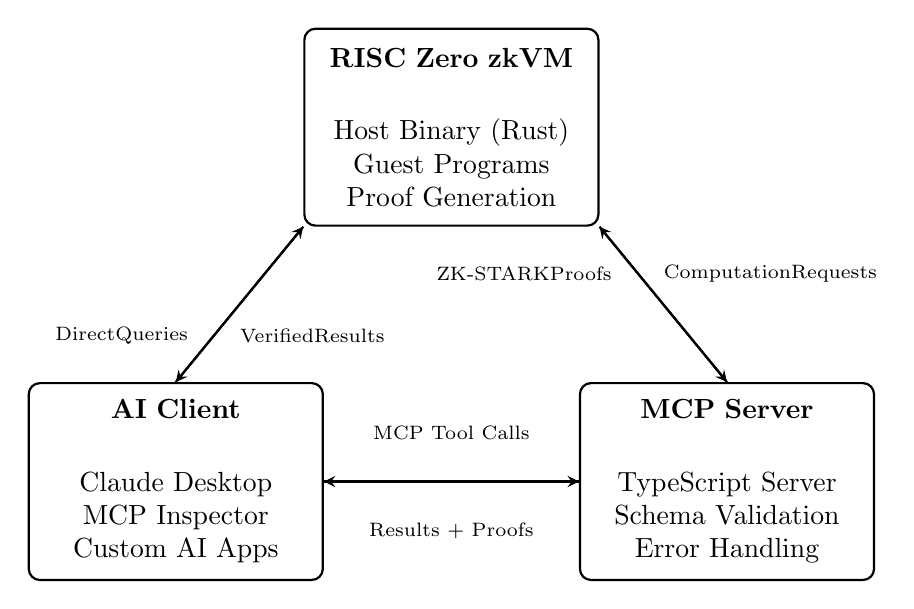
\begin{tikzpicture}[auto]
  % Define styles
  \tikzstyle{system} = [rectangle, draw, text width=3.5cm, text centered, rounded corners, minimum height=2.5cm, thick]
  \tikzstyle{arrow} = [thick,->,>=stealth]
  \tikzstyle{label} = [font=\scriptsize, text centered]
  
  % Main system components in triangular layout with more spacing
  \node [system] (client) at (0,0) {
    \textbf{AI Client}\\[0.5cm]
    Claude Desktop\\
    MCP Inspector\\
    Custom AI Apps
  };
  
  \node [system] (mcpserver) at (7,0) {
    \textbf{MCP Server}\\[0.5cm]
    TypeScript Server\\
    Schema Validation\\
    Error Handling
  };
  
  \node [system] (risc0) at (3.5,4.5) {
    \textbf{RISC Zero zkVM}\\[0.5cm]
    Host Binary (Rust)\\
    Guest Programs\\
    Proof Generation
  };
  
  % Arrows with labels for data flow - with proper spacing
  \draw [arrow] (client.east) -- (mcpserver.west) node[midway, above, label, yshift=4mm] {MCP Tool Calls};
  \draw [arrow] (mcpserver.west) -- (client.east) node[midway, below, label, yshift=-4mm] {Results + Proofs};
  
  \draw [arrow] (mcpserver.north) -- (risc0.south east) node[pos=0.7, right, label, xshift=2mm] {Computation\\Requests};
  \draw [arrow] (risc0.south east) -- (mcpserver.north) node[pos=0.3, left, label, xshift=-2mm] {ZK-STARK\\Proofs};
  
  \draw [arrow] (client.north) -- (risc0.south west) node[pos=0.3, left, label, xshift=-2mm] {Direct\\Queries};
  \draw [arrow] (risc0.south west) -- (client.north) node[pos=0.7, right, label, xshift=2mm] {Verified\\Results};
  
\end{tikzpicture}
\caption{RISC Zero MCP System Architecture with Data Flow}
\label{fig:architecture}
\end{figure}
\subsection{AI Client}


The AI Client component encompasses applications like Claude Desktop, MCP Inspector, and custom AI applications that consume zero-knowledge proof functionality through standardized MCP protocols. These clients provide tool discovery capabilities that automatically detect and register available zkVM operations, request formatting that validates input parameters and prepares them for transmission to the MCP server, and result processing that interprets proof artifacts and extracts computational results for presentation to end users. The clients support both interactive and programmatic access patterns, enabling AI agents to seamlessly integrate zero-knowledge proof generation into their workflows while maintaining familiar interaction paradigms. The standardized MCP interface ensures broad compatibility across different client implementations, allowing the same proof generation capabilities to be accessed from various AI applications and platforms.

\subsection{MCP Server}

The MCP Server acts as the orchestration layer, implemented as a TypeScript server that manages proof generation workflows and serves as the bridge between AI clients and the underlying cryptographic system. The server exposes ten primary tools to AI clients: mathematical operations including zkvm\_add, zkvm\_multiply, zkvm\_sqrt, zkvm\_modexp, and zkvm\_range for range proofs; machine learning capabilities including zkvm\_k\_means, zkvm\_linear\_regression, zkvm\_neural\_network, and zkvm\_logistic\_regression for privacy-preserving statistical analysis; and verify\_proof for independent verification of computational integrity. The server implements comprehensive schema validation to ensure input parameters meet cryptographic requirements, robust error handling with meaningful error messages for debugging, and asynchronous processing with appropriate timeout management to prevent resource exhaustion. Each tool follows the MCP specification with structured input schemas and standardized response formats containing computational results, proof metadata, and verification status.

\subsection{RISC Zero Integration Layer}

This layer provides the core integration with RISC Zero's zkVM system:

The RISC Zero Integration Layer provides the core integration with RISC Zero's zkVM system through four essential components that handle all low-level cryptographic operations. Guest Program Management maintains and executes specialized RISC-V programs for each supported operation, ensuring that computational logic is properly isolated and executed within the zkVM environment, while Proof Generation orchestrates the zkVM execution and STARK proof generation process, coordinating the complex sequence of operations required to produce cryptographic proofs. The Verification Interface provides standardized interfaces for proof verification, abstracting the complexity of cryptographic validation from higher-level components, and Performance Optimization implements caching and optimization strategies to improve proof generation performance, reducing computational overhead and improving system responsiveness.

\subsection{RISC Zero zkVM}

The RISC Zero zkVM component encompasses the core cryptographic infrastructure, including Rust-based host binaries, specialized guest programs, and proof generation capabilities that execute computations and generate ZK-STARK proofs. The host binary orchestrates zkVM execution and manages the proof generation workflow, configuring the executor environment with appropriate inputs and coordinating the complex sequence of cryptographic operations required to produce valid proofs. Guest programs are specialized RISC-V executables developed for each supported operation, implementing fixed-point arithmetic for decimal operations, optimized algorithms for machine learning computations, and comprehensive input validation to ensure mathematical correctness. The system includes dedicated guest programs for K-means clustering with distance calculations and centroid updates, linear regression with least squares optimization, neural network inference with pre-trained weights and sigmoid activation, and logistic regression for privacy-preserving binary classification. Proof generation produces cryptographic artifacts that verify computational correctness while maintaining privacy of sensitive inputs, and verification capabilities validate generated proofs against expected image identifiers to ensure authenticity and integrity.

\section{Agent-to-Agent Verification Workflow}
\label{sec:agent-verification}

To demonstrate the practical application of our system in cross-party agentic workflows, we present a concrete example of AI agents performing logistic regression with zero-knowledge proof verification. Figure~\ref{fig:agent-workflow} illustrates the interaction between a Prover Agent and a Verifier Agent, showcasing how one AI agent can verify machine learning computations performed by another agent without accessing sensitive training data or model parameters.

\begin{figure}[ht]
\centering
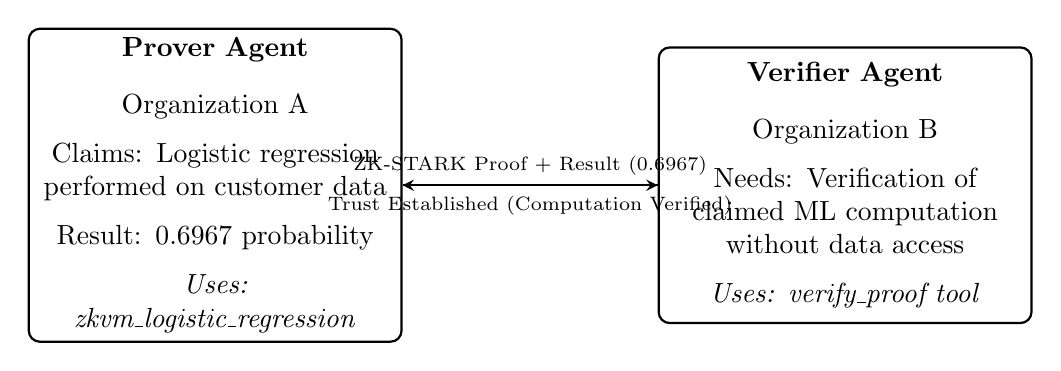
\begin{tikzpicture}[auto, node distance=8cm]
  % Define styles
  \tikzstyle{agent} = [rectangle, draw, text width=4.5cm, text centered, rounded corners, minimum height=3.5cm, thick]
  \tikzstyle{arrow} = [thick,->,>=stealth]
  \tikzstyle{label} = [font=\scriptsize, text centered]
  
  % Agents
  \node [agent] (prover) at (0,0) {
    \textbf{Prover Agent}\\[0.3cm]
    Organization A\\[0.2cm]
    Claims: Logistic regression\\
    performed on customer data\\[0.2cm]
    Result: 0.6967 probability\\[0.2cm]
    \textit{Uses: zkvm\_logistic\_regression}
  };
  
  \node [agent] (verifier) at (8,0) {
    \textbf{Verifier Agent}\\[0.3cm]
    Organization B\\[0.2cm]
    Needs: Verification of\\
    claimed ML computation\\
    without data access\\[0.2cm]
    \textit{Uses: verify\_proof tool}
  };
  
  % Workflow arrows
  \draw [arrow] (prover.east) -- (verifier.west) node[pos=0.5, above, label] {ZK-STARK Proof + Result (0.6967)};
  \draw [arrow] (verifier.west) -- (prover.east) node[pos=0.5, below, label] {Trust Established (Computation Verified)};
  
\end{tikzpicture}
\caption{Agent-to-Agent Zero-Knowledge Proof Verification Workflow for Logistic Regression}
\label{fig:agent-workflow}
\end{figure}

The workflow demonstrates four key stages of cross-party agent verification:

\textbf{Stage 1: Proof Generation} - The Prover Agent executes the logistic regression computation using our system's zkvm\_logistic\_regression tool, which generates a ZK-STARK proof of the computation while keeping the training data and model parameters completely private. This corresponds to running `npm run test:logistic-regression` in our implementation.

\textbf{Stage 2: Proof Transmission} - The Prover Agent transmits both the computational result (probability value 0.6967) and the accompanying ZK-STARK proof to the Verifier Agent. The proof serves as cryptographic evidence that the computation was performed correctly without revealing any sensitive information about the underlying data or model architecture.

\textbf{Stage 3: Verification} - The Verifier Agent uses the verify\_proof tool to validate the received proof, confirming that the claimed logistic regression computation was indeed performed correctly and that the reported probability value is authentic. This verification process is computationally efficient (typically 15-25ms) and requires no access to the original training data.

\textbf{Stage 4: Trust Establishment} - Upon successful verification, trust is established between the agents. The Verifier Agent can confidently rely on the Prover Agent's machine learning results without requiring access to proprietary datasets or model parameters, enabling secure cross-organizational AI collaboration.

This workflow exemplifies how our RISC Zero MCP system enables trustless computation verification in multi-party AI scenarios, addressing the critical challenge of verifiable computation in autonomous agent systems while maintaining privacy and competitive advantages.

\section{Evaluation}
\label{sec:evaluation}

\subsection{Performance Analysis}

We conducted comprehensive performance evaluation across multiple dimensions:

\textbf{Proof Generation Time}: We conducted comprehensive performance evaluation across multiple dimensions, with Table~\ref{tab:performance} showing proof generation times for different operations where complex operations like modular exponentiation require more time due to increased computational complexity.

\begin{table}[ht]
\centering
\caption{Proof Generation Performance}
\label{tab:performance}
\begin{tabular}{lrr}
\toprule
Operation & Mean Time (ms) & Std Dev (ms) \\
\midrule
Addition & 3,247 & 145 \\
Multiplication & 3,398 & 178 \\
Square Root & 3,521 & 203 \\
Modular Exponentiation & 4,127 & 267 \\
Range Proof & 3,876 & 198 \\
\bottomrule
\end{tabular}
\end{table}

\textbf{Storage Efficiency}: Our binary proof format achieves significant storage savings compared to traditional approaches, with the binary format requiring approximately 210KB per proof while the hexadecimal format requires approximately 420KB per proof, resulting in a storage reduction of approximately 50% that directly translates to reduced storage costs and faster proof transmission over networks.

\textbf{Verification Performance}: Proof verification demonstrates consistently fast performance across all operation types, typically completing in 15-25ms regardless of the original computation complexity, indicating that verification overhead remains minimal even for complex cryptographic operations.

\subsection{Integration Testing}

We validated MCP integration through comprehensive testing:

We validated MCP integration through comprehensive testing across multiple dimensions to ensure broad compatibility and reliable operation. Client Compatibility testing successfully validated operation with multiple MCP clients including Claude Desktop and custom implementations, demonstrating the system's adherence to MCP specifications and broad interoperability, while Tool Discovery verification confirmed automatic tool discovery and schema validation across different client implementations, ensuring seamless integration regardless of client-specific variations. Error Handling testing confirmed robust error propagation and handling across the MCP interface, validating that error conditions are properly communicated and handled throughout the entire system stack.

\section{Conclusion}
\label{sec:conclusion}

This paper presents RISC Zero MCP, a comprehensive system that bridges zero-knowledge proof generation and AI tool integration through the Model Context Protocol. Our implementation demonstrates that complex cryptographic systems can be made accessible to AI applications through standardized interfaces, enabling new paradigms for privacy-preserving and verifiable computation. Our evaluation shows that the system provides great performance characteristics while maintaining cryptographic security guarantees. As AI systems become more autonomous and handle increasingly sensitive data, the integration of cryptographic proof systems becomes essential. Our work provides a foundation for this integration, demonstrating practical approaches and identifying key considerations for future development.

\end{document}